\documentclass[prb]{revtex4}
%\documentclass[a4paper,10pt]{article}


%%%%%%%Specific packages%%%%%%%%%%%%%
\usepackage[usenames,dvipsnames]{color}

\usepackage{pdfpages}
\usepackage[british]{babel} 
%\usepackage[svgnames,x11names]{xcolor}
%\usepackage{graphics}
\usepackage{mathtools}
\usepackage{braket}

\usepackage[b]{esvect} % Vector notation 
\usepackage{empheq}    % boxed equation 

\usepackage{amssymb}
\usepackage{amsfonts}
\usepackage{amsmath}
\usepackage{graphicx}
\usepackage{textcomp}   % text companion fonts
%\usepackage{dcolumn}
\usepackage{bm}         % bold math
\usepackage{microtype}  % makes pdf looks better
%\usepackage{lmodern}
%\fontfamily{garamond}
%\fontfamily{\familydefault}
%\renewcommand*\familydefault{\sfdefault} %% Only if the base font of the document is to be sans serif
%\usepackage[sf]{titlesec}

%\usepackage{mathrsfs}
%\usepackage{bbold}
%\usepackage{epsfig}
%\usepackage{booktabs}    % table format 
%\usepackage{wasysym}
%\usepackage{pmat}       % also matrix partition 
%\usepackage{fancybox} 
%\usepackage{subfig}      % figure side by side
%\usepackage{sidecap}     % side caption
%\usepackage{setspace}    % for line spacing 
%\usepackage{ctable}      % better table spacing
%\usepackage[OT1]{fontenc} % font 
%\usepackage{helvet}      % Helvetica
\usepackage{mathptmx}    % Times 
%\usepackage[sc,osf]{mathpazo}
%\usepackage[version=3]{mhchem} % chemical formulas 
%\usepackage{showkeys}    % switch it off when not needed.
%\usepackage{flafter}    % place figures/tables after references in text 
%\usepackage[left=1.5in, right=1in, top=1in, bottom=1in, includefoot,
 %                    headheight=13.6pt]{geometry}   % changing the page layout  
%\usepackage[latin1]{inputenc}
%\usepackage{euler}       % Font for math mode 
%\setlength{\abovecaptionskip}{5pt}
\usepackage[breaklinks]{hyperref} %%% Hyper-linking
\hypersetup{colorlinks=false}

%%% paragraph setting
\setlength{\parskip}{2.0ex plus 0.2ex minus 0.2ex}
\setlength{\parindent}{0pt}
\renewcommand{\arraystretch}{2.0}


%%% hack boxed 
\newcommand*{\boxedcolor}{Lavender}

\definecolor{mycol}{RGB}{255, 229, 255}
\newcommand*\mybox[1]{\colorbox{mycol}{\hspace{1em}#1\hspace{1em}}}

\makeatletter
\renewcommand{\boxed}[1]{\textcolor{\boxedcolor}{%
\fbox{\normalcolor\m@th$\displaystyle#1$}}}
\makeatother

%%% Few specific commands  %%%
\newcommand{\eq}[1]{\begin{align}#1\end{align}}

\newcommand{\ba}{\begin{array}}
\newcommand{\ea}{\end{array}}

\newcommand{\bit}{\begin{itemize}}
\newcommand{\eit}{\end{itemize}}

\newcommand{\br}{{\bf r}}
\newcommand{\Le}{\left}
\newcommand{\Ri}{\right}
\newcommand{\nn}{\nonumber}
\newcommand{\R}{\rho}
\newcommand{\f}{\frac}
\newcommand{\bs}{\boldsymbol}
\newcommand{\B} {\bf}
\newcommand{\mbf}{\mathbf}
\newcommand{\mrm}{\mathrm}
\newcommand{\tr}{\textrm}
\newcommand{\tbl}{\textcolor{blue}}
\newcommand{\trd}{\textcolor{red}}
\newcommand{\mc}{\mathcal}
\newcommand{\mf}{\mathfrak}
\newcommand{\dg}{\dagger}
\newcommand{\om}{\omega}
\newcommand{\ra}{\rangle}
\newcommand{\la}{\langle}
\newcommand{\ua}{\uparrow}
\newcommand{\da}{\downarrow}

\newcommand{\ii}{i}
\newcommand*\conj[1]{{#1^\star}}
\newcommand*\conjk[1]{{#1^{k\star}}}
\newcommand*\conjp[1]{{#1^{p\star}}}
\newcommand*\dotconjp[1]{{\dot{#1}^{p\star}}}
\newcommand*\dotp[1]{{\dot{#1}^{p}}}
\newcommand*\p[1]{{\dot{#1}^{p}}}
\newcommand*\kp{\boldsymbol{\kappa}}
\newcommand{\wk}{\omega_k}

\newcommand{\ff}[2]{\la f_{#1} | f_{#2} \ra}
\newcommand{\fg}[2]{\la f_{#1} | h_{#2} \ra}
\newcommand{\gf}[2]{\la h_{#1} | f_{#2} \ra}
\newcommand{\ggnm}[2]{\la h_{#1} | h_{#2} \ra}

%\newcommand{\fm}{f_m}
%\newcommand{\pj}{p_j}
%\newcommand{\pm}{p_m}

% begin document
\begin{document}
\title{Dynamical equations of a qubit coupled to a cavity decaying into a bosonic bath -- via SPIN-BOSON}
\author{Nicolas Gheeraert}
\date{\today}
\maketitle
%%%%%%%%%%%%%%%%%%%%%%%%%%%%%%%%%%%%%%%%%%%%%%%%%%%%%%%%%%%%%%%%
%\begin{center}
%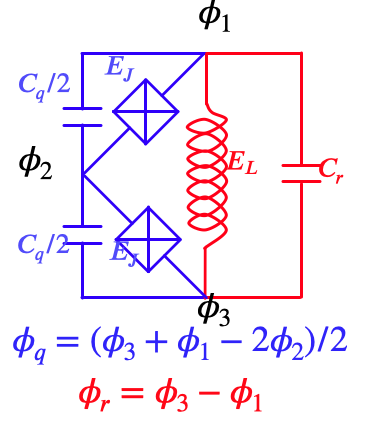
\includegraphics[scale=0.25]{circuit_diagram}
%\end{center}
%
The quantromon Lagrangian is given by:
\eq{
L= \frac{1}{2} \left( \frac{C_q}{2} \right) \dot \Phi_1^2  +  \frac{1}{2} \left( \frac{C_q}{2} \right) \dot \Phi_3^2 +  \frac{1}{2} C_r (\dot \Phi_3 - \dot \Phi_1)^2   +E_J \cos\left(\frac{\Phi_1}{\phi_0}\right) +E_J \cos\left(\frac{\Phi_3}{\phi_0}\right) - \frac{1}{2L}\left(\Phi_1-\Phi_3-\Phi\right)^2
}
%
Defining $\Phi_q = \frac{1}{2} ( \Phi_1 + \Phi_3 )$, and $\Phi_q = \frac{1}{2} ( \Phi_1 - \Phi_3 )$, we get:
%
\eq{
L=\frac{1}{2} C_q\dot \Phi_q^2  +  \frac{1}{2} ( C_q +  4 C_r ) \dot \Phi_r^2   +2E_J \cos\left(\frac{\Phi_q}{\phi_0}\right)\cos\left(\frac{\Phi_r}{\phi_0}\right) - \frac{2}{L}\left(\Phi_r-\Phi/2 \right)^2
}
The quantromon Hamiltonian is given by:
%
\eq{
H= \frac{Q_q^2}{2C_q} +  \frac{Q_r^2}{2(C_q+4 C_r)}  - 2 E_J \cos\left(\frac{\Phi_q}{\phi_0}\right)\cos\left(\frac{\Phi_r}{\phi_0}\right) + \frac{2}{L}(\Phi_r-\Phi/2)^2
}
%
Defining $E_{C_q} \equiv e^2/(2C_q)$, $E_{C_r} \equiv e^2/(2(4C_r+C_q))$, $E_{L_r} \equiv 4\phi_0^2/L$, and setting $\Phi=0$, we get:
%
\eq{
H= 4 E_{C_q} n_q^2 + 4E_{C_r} n_r^2 - 2E_J \cos(\varphi_q)\cos(\varphi_r) + \frac{E_{L_r}}{2} \varphi_r^2
}
Linearising the cavity cosine:
%
\eq{
H= 4 E_{C_q} n_q^2 - 2E_J \cos(\varphi_q)+ 4E_{C_r} n_r^2 +E_J \cos(\varphi_q)\varphi_r^2 + \frac{E_{L_r}}{2} \varphi_r^2
}
%
Define the resonator ladder operators such that:
\eq{
\varphi_r &= \left( \frac{2E_{C_r}}{E_{L_r}} \right)^{1/4} ( a^\dag + a ) = \sqrt{\eta_r} ( a^\dag + a ) \quad \quad {\rm where}  \quad \quad \eta_r= \sqrt{\frac{2E_{C_r}}{E_{L_r}}}  \notag \\
 n_r &= i\left( \frac{E_{L_r}}{32E_{C_r}} \right)^{1/4}  ( a^\dag - a) 
 }
Defining $\omega_r=\sqrt{8E_{C_r}E_{L_r}}$, we get:
%
\eq{
H= 4 E_{C_q} n_q^2 - 2E_J \cos(\varphi_q)+ \omega_r a^\dag a + E_J\eta_r\cos(\varphi_q)(a^2 + {a^\dag}^2 +  2 a^\dag a +1 ),
}
Defining the transmon effective Josephson energy $E_{J_q} = E_J(2 - \eta_r)$:
%
\eq{
H= 4 E_{C_q} n_q^2 - E_{J_q} \cos(\varphi_q) + \omega_r a^\dag a + E_J\eta_r \cos(\varphi_q)(a^2 + {a^\dag}^2 +  2 a^\dag a ),
}
Defining the transmon ladder operators such that:
\eq{
\varphi_q &= \left( \frac{2E_{C_q}}{E_{J_q}} \right)^{1/4} ( q^\dag + q ) = \sqrt{\eta_q} ( q^\dag + q ) \quad \quad {\rm where}  \quad \quad \eta_q= \sqrt{\frac{2E_{C_q}}{E_{J_q}}}  \notag \\
 n_q &= i\left( \frac{E_{J_q}}{32E_{C_q}} \right)^{1/4}  ( q^\dag - q ) 
 }
Defining , and $g_{q-r} \equiv E_J\eta_r$:
%
\eq{
H= 4 E_{C_q} n_q^2 - E_{J_q} \cos(\varphi_q) + \omega_r a^\dag a + g_{q-r}\cos(\varphi_q)(a^2 + {a^\dag}^2 +  2 a^\dag a ),
}
Rewriting the transmon operators in its eigenbasis, adding drive and decay, the full Hamiltonian becomes:
%
\eq{
\hat H = \sum_{i=0}^{N_q-1} \omega_{\rm qb }^i \ket{i} \bra{i} &+ \omega_r a^\dag a  + \sum_{i,j} g_{ij}\ket{i}\bra{j} (a^2 + {a^\dag}^2 +  2 a^\dag a ) \notag \\
&+\sum_{k=1}^{N} \omega_k \hat d_k^\dag \hat d_k +a^\dag \sum_{k=1} \gamma_k d_k+a \sum_{k=1} \gamma_k^\star d_k^\dag  \notag \\
&+A_{\rm d} \cos(\omega^{\rm drive}t) (a+a^\dag)
}
where $g_{ij} = g_{q-r} \braket{ i | \cos(\varphi_q) | j } $.

%%%%%%%%%%%%%%%%%%%%%%%%%%%%%%%%%%%%%%%%%%%%%%%%%%%%%%%%
%%%%%%%%%%%%%%%%%%%%%%%%%%%%%%%%%%%%%%%%%%%%%%%%%%%%%%%%

\section{ Diagonalisation of the free bosonic modes }

%%%%%%%%%%%%%%%%%%%%%%%%%%%%%%%%%%%%%%%%%%%%%%%%%%%%%%%%
%%%%%%%%%%%%%%%%%%%%%%%%%%%%%%%%%%%%%%%%%%%%%%%%%%%%%%%%

By combining the field modes together:
\eq{
&a_0^\dag \equiv a^\dag \quad \text{if}\quad  p=k=0,\\
&a_p^\dag \equiv d_k^\dag \quad \text{if}\quad  p=k \ne 0,
}
we can obtain:
\eq{
H = \sum_{i=0}^{ N_q-1} \omega_{\rm qb }^i \ket{i} \bra{i}  + \Big( a_0^2+(a_0^\dag)^2 +  a_0^\dag a_0 \Big)  \sum_{i,j}^{\ N_q-1} g^{\rm qb-cav}_{i,j}\ket{i}\bra{j} + \sum_{p,p'} h_{p p'} a_p^\dag a_{p'} + A(t) (a_0+a_0^\dag) ,
}
with 
\eq{
h_{00} &= \omega_{\rm cav} \notag\\
h_{kk} &= \omega^k_{\rm bath} \notag\\
h_{0k} &= h_{k0}^\star =  \gamma_k \notag\\
h_{pp'} &= 0 \quad {\rm else}.
}

Diagonalising the matrix $h_{pp'}$ provides normal modes $b_p$ of the problem:
\eq{
\sum_{pp'} h_{pp'} a_p^\dag a_{p'} = \sum_p \omega_p b_p^\dag b_p,
}
In doing so, we have defined the ladder operators in in the new basis:
\eq{
b_\sigma = \sum_\mu O^T_{\sigma \mu} a_\mu
}
Conversely,
\eq{
a_0 = \sum_\mu O_{0\mu} b_\mu \quad \text{and} \quad a_k = \sum_\mu O_{k \mu} b_\mu.
}
The matrix $O$ denotes the transfer matrix used to go from the original basis to the new basis. It verifies:
\eq{
D = O^T h O.
}
Hence we obtain the following Hamiltonian:
\eq{
H & = \sum_{i=0}^{ N_q-1} \omega_{\rm qb }^i \ket{i} \bra{i}  + \Big( a_0^2+(a_0^\dag)^2 +  a_0^\dag a_0 \Big)  \sum_{i,j}^{\ N_q-1} g^{\rm qb-cav}_{i,j}\ket{i}\bra{j} + \sum_{p}\omega_p b_p^\dag b_p +  A(t) \sum_p O_{0p}(b_p+b_p^\dag),
}
where we have defined the coupling $g_{i,i+1}^p$ between the transmon and the normal-mode $p$  as 
\eq{
g_{i,j}^p = g^{\rm qb-cav}_{i,j} O_{0p}.
}

\section{General algorithm}


%
We start with the following wavefunction
\eq{
|\Psi\ra = \sum_{i}^{N_q-1} \sum_{n}^{\rm ncs} p_{i,n} \ket{i} \ket{z_{i,n}}
}
Here $p_{i,n}$ and $z_{i,n}^p$ are all complex and time dependent variational parameters. 

The Lagrangian is given by:

\eq{
\mc{L}  = \braket{ \Psi | \frac{i}{2}  \overleftrightarrow{\partial_t} - \hat H | \Psi  }
}

Explicitely:

\eq{
\braket{\Psi|  \vv*{\partial}{t} | \Psi } 
&=  \left(\sum_{m} p_m^\star  \bra{z_m} \right) \vv*{\partial}{t} \left(\sum_{n} p_n \ket{z_n} \right)  \notag \\
&= \sum_{mn} p_m^\star  \braket{z_m|z_n} \biggl( \dot{p}_n -\frac{1}{2}p_n \Bigl( \sum_p \dot{z}_n^p z_n^{p\star} + z_n^p \dot{z}_n^{p\star} - 2 z_m^{p\star} \dot{z}_n^p \Bigr)  \biggr)
}
where we have used: 
\eq{
\la z_n | \vv*{\partial}{t} | z_m \ra &= -\f{1}{2} \Le( \sum_p  \dot{z}_m^p z_m^{p\star} +
z_m^p \dot{z}_m^{p\star} -2 z_n^{p\star}\dot{z}_m^p \Ri) \la z_n | z_m \ra \nn 
}
Since we have that:
\eq{
\braket{\Psi|   \overleftarrow{\partial_t} | \Psi }  =  \braket{\Psi| \overrightarrow{\partial_t} | \Psi } ^\star,
}
we obtain:
\eq{
\mc{L}  &= \frac{i}{2}\sum_{mn}  \braket{z_m|z_n} \biggl[ p_m^\star \dot{p}_n - p_n \dot{p}_m^\star - \frac{1}{2}p_m^\star p_n \Bigl( \sum_p \dot{z}_n^p z_n^{p\star} + z_n^p \dot{z}_n^{p\star} - 2 z_m^{p\star} \dot{z}_n^p - \dot{z}_m^{p\star} z_m ^p- z_m^{p\star} \dot{z}_m^p + 2 z_n^p \dot{z}_m^{p\star} \Bigr)  \biggr] -  \braket{ \Psi |  \hat H | \Psi  }
}

The Euler-Lagrange equations are: 
\eq{
\f{d}{d t} \f{\partial \mc{L}}{\partial \conj{\dot{p}_j}} - \f{\partial
\mc{L}}{\partial \conj{p_j}} =0  \quad \text{and} \qquad
\f{d}{d t} \f{\partial
\mc{L}}{\partial \conjp{\dot{z}_j}} - \f{\partial
\mc{L}}{\partial \conjp{z_j}} =0.
}

After $\conj{p_j}$ variation we get
\begin{empheq}[box=\fbox]{equation}
 \sum_m \Le( \dot{p}_m - \frac{1}{2}p_m \kp_{mj} \Ri) M_{jm} = -\ii \f{\partial E}{\partial \conj{p_j}}  \equiv P_j
\label{equation1}
\end{empheq}

After $\conjp{z_j}$ variation we get
\eq{
  \sum_m p_m \conj{p_j} \dot{z}_m^p  M_{jm}
-\f{1}{4} \sum_m \Le(2 \dot{p}_m - p_m \kp_{mj}  \Ri) \conj{p_j} (z_j^p-2z_m^p)
M_{jm} 
+\f{1}{4} \sum_m \Le(2 \conj{\dot{p}_m} - \conj{p_m}\conj{\kp_{mj}} \Ri) p_j
z_j^p M_{mj} = -i \f{\partial E}{\partial \conjp{z_j}}
\label{rawequation2_B}
}
where we have defined:
\eq{
&M_{jm} = \braket{z_j|z_m} \\
&\kappa_{mj} =  \sum_p \dot{z}_m^p z_m^{p\star} + \dot{z}_m^{p\star} z_m^p - 2 z_j^{p\star} \dot{z}_m^p
}
Using (\ref{equation1}) to simplify (\ref{rawequation2_B}), we get:
\begin{empheq}[box=\fbox]{equation}
\sum_m p_m  \dot{z}_m^p M_{jm}  + \sum_m ( \dot{p}_m
- \f{1}{2} p_m \kp_{mj})  z_m^p M_{jm}  =  Z_j^p,
\label{equation2_Z}
\end{empheq}
where we have defined:
\eq{
Z_j^p = -\ii \Le[\f{\partial E}{\partial \conjp{z_j}}\frac{1}{p_j^\star}  + \f{1}{2} \Le( \f{\partial E}{\partial p_j^\star}
 + \f{\partial E}{\partial p_j } \frac{p_j}{p_j^\star}  \Ri) z_j^p \Ri] 
}
From here on we only derive the equations for $\dot{y}_n$, as those $\dot{z}_n^p$ can be guessed from the former.

From  Eqs. (\ref{equation1}) and (\ref{equation2_Z}), we get:
\eq{
\sum_j M_{nj}^{-1} P_j &= \dot{p}_n - \frac{1}{2}\sum_{mj} p_m \kappa_{mj}M_{nj}^{-1}M_{jm} \notag \\
&=  \dot{p}_n - \frac{1}{2} p_n \Big(  \sum_q \dot{z}_n^q z_n^{q\star} + \dot{z}_n^{q\star} z_n^q \Big) + \sum_{mj} M_{nj}^{-1}M_{jm} p_m \Big( \sum_q z_j^{q\star} \dot{z}_m^q\Bigr) \label{eq_int_1} \\
%
\sum_j M_{nj}^{-1} Z_j^p &= p_n \dot{z}_n^p + \dot{p}_n z_n^p - \frac{1}{2} p_n z_n^p \Big(   \sum_q \dot{z}_n^q z_n^{q\star} + \dot{z}_n^{q\star} z_n^q \Big) + \sum_{mj} M_{nj}^{-1}M_{jm} p_m z_m^p\Big( \sum_q z_j^{q\star} \dot{z}_m^q\Big)
 \label{eq_int_3}
}
From here we can obtain:
\eq{
\sum_j M_{nj}^{-1} Z_j^p - z_n^p \sum_j M_{nj}^{-1} P_j  = p_n \dot{z}_n^p + \sum_{mj} M_{nj}^{-1}M_{jm} p_m \Big( \sum_q z_j^{q\star} \dot{z}_m^q\Bigr) (z_m^p-z_n^p) \label{eq_int_5}.
}
Hence:
\eq{
z_i^{p\star}\sum_j M_{nj}^{-1} \Big( Z_j^p - z_n^p  P_j\Big)  = p_n z_i^{p\star}\dot{z}_n^p + \sum_{mj} M_{nj}^{-1}M_{jm} p_m \Big( \sum_q z_j^{q\star} \dot{z}_m^q\Bigr) (z_i^{p\star}z_m^p-z_i^{p\star}z_n^p) \label{eq_int_7}.
}
Defining:
\eq{
&a_{in} = p_n\Big(  \sum_p z_i^{p\star} \dot{z}_n^p \Big), \\
&b_{in} = \sum_p z_i^{p\star} z_n^p, \\
&A_{in} =  \sum_j M_{nj}^{-1} \Big(  \sum_p z_i^{p\star}(Z_j^p - z_n^p P_j )  \Big),
}
we obtain an equation from Eq. (\ref{eq_int_5}) which do not depend on the mode index:
\begin{empheq}[box=\fbox]{equation}
a_{in} + \sum_{mj} M_{nj}^{-1} M_{jm}a_{jm}  ( b_{im} - b_{in} ) = A_{in} \label{ain_equation}.
\end{empheq}


In order to solve (\ref{ain_equation}), we define:
\eq{
d_{in}  \equiv \sum_l M_{il}^{-1} M_{ln} a_{ln},
}
and use it to reexpress (\ref{ain_equation}):
\eq{
d_{in} + \sum_m\left( \sum_l M_{il}^{-1} M_{ln} (b_{lm} -b_{ln})  \right)d_{nm} = \sum_l M_{il}^{-1} M_{ln} A_{ln}
}
Hence we get:
\begin{empheq}[box=\fbox]{equation}
\sum_{mj}( \delta_{mn}\delta_{ij} +\alpha_{inm} \delta_{jn} ) d_{jm} = \sum_l M_{il}^{-1} M_{ln} A_{ln}
\label{alpha_equation}
\end{empheq}
where:
\eq{
\alpha_{inm} = \sum_l M_{il}^{-1} M_{ln} (b_{lm} - b_{ln} )
}
Once we have solved for $d_{in}$, we get $\dot{z}_n^p$ and $\dot{p}_n$  from Eqs. (\ref{eq_int_1}) and (\ref{eq_int_5}):
\begin{empheq}[box=\fbox]{align}
&\dot{p}_n = \sum_j M_{nj}^{-1} P_j + \frac{1}{2} p_n \Big( \sum_q \dot{z}_n^q z_n^{q\star} + \dot{z}_n^{q\star} z_n^q \Big)  - \sum_m d_{nm} \\
&\dot{z}_n^p = \frac{1}{p_n}\left( \sum_j M_{nj}^{-1} (Z_j^p -  z_n^p P_j) - \sum_{m}  d_{nm}(z_m^p-z_n^p)   \right)
\end{empheq}

\section{Relevant term evaluations}

Let us now evaluate the terms on the RHS of the two dynamical equations. \\

First, the energy is given by:
\eq{	
E =& \Big(  \sum_{l,m} p_{l,m}^\star \bra{l} \bra{z_{l,m}}\Big) H \Big(  \sum_{i,n} p_{i,n}\ket{i} \ket{z_{i,n}}\Big)  \notag \\
E=& \sum_{i,n,m}  p_{i,m}^{\star} p_{i,n}  \braket{ z_{i,m} | z_{i,n} } \Bigl[\omega^{\rm qb}_i  +\sum_{p=0} \omega_p z_{i,m}^{p\star} z_{i,n}^p + A(t)\sum_{p} O_{0,p}\Big( z_{i,m}^{p\star} +z_{i,n}^{p}  \Big)   \Bigr]  \notag \\
&+  \sum_{i,l,n,m}  g_{li}  p_{l,m}^{\star} p_{i,n}  \braket{ z_{l,m} | z_{i,n} } \big( z_{l,m}^{0\star} + z_{i,n}^{0}  \big)^2
}
%
\eq{	
\frac{\partial E}{\partial p_{s,j}^\star} =& \sum_{n}   p_{s,n} \braket{ z_{s,j} | z_{s,n} } \Bigl[ \omega^{\rm qb}_s  +  \sum_p \omega_p z_{s,j}^{p\star} z_{s,n}^p  + A(t)\sum_{p} O_{0,p}\Big( z_{s,j}^{p\star} + z_{s,n}^{p}  \Big) \Bigr] \\ 
&+  \sum_{i,n}  g_{si}  p_{i,n}  \braket{ z_{s,j} | z_{i,n} } \big( z_{s,j}^{0\star} + z_{i,n}^0 \big)^2
\\
%
\frac{\partial E}{\partial z_{s,j}^{q\star}} =&\sum_{n}   p_{s,j}^\star p_{s,n} \braket{ z_{s,j} | z_{s,n} }  \Bigl[ \omega_q z_{s,n}^{q} 
+ A(t) O_{0,q} +( z_{s,n}^{q} - \tfrac{1}{2}z_{s,j}^{q} ) \Big(\omega_s^{\rm qb} + \sum_{k=0} \omega_p z_{s,j}^{p\star} z_{s,n}^p + A(t)\sum_{p} O_{0,p}\big(z_{s,j}^{p\star} + z_{s,n}^{p}\big) \Big) \Big] \notag \\
& - \frac{1}{2} \sum_n p_{s,n}^\star p_{s,j}  \braket{z_{s,n}|z_{s,j}} z_{s,j}^{q} \Big[  \omega_{\rm s}^{\rm qb} + \sum_{p=0}  \omega_p z_{s,n}^{p\star} z_{s,j}^p + A(t)\sum_{p} O_{0,p}\big(z_{s,n}^{p\star} + z_{s,j}^{p}\big)  \Big] \notag\\
&+\sum_{in} \Big[  p_{s,j}^\star p_{i,n} \braket{z_{s,j} |z_{i,n} } \Big(2 g_{s,i}O_{0,q}(z_{s,j}^{0 \star} +z_{i,n}^{0} ) + (z_{i,n}^{q} - \tfrac{1}{2}z_{s,j}^{q}) g_{s,i}  \big( z_{s,j}^{0\star} + z_{i,n}^{0}  \big)^2  \Big) \\
& \hspace{1cm}- \frac{1}{2}p_{i,n}^\star p_{s,j}  \braket{z_{i,n}|z_{s,j}} z_{s,j}^{q}  g_{i,s} \big( z_{i,n}^{0\star} + z_{s,j}^{0} \big)^2 \Big] 
}

\section{Evaluating the error between the polaron ansatz and the exact solution}

To check the accuracy of our wave-function, we monitor the norm of the following vector:

\begin{equation}
\ket{\Phi} =  \biggl( i \frac{\overset{\rightarrow}{\partial_t}}{2} - i \frac{\overset{\leftarrow}{\partial_t}}{2} - H \biggr) \ket{ \Psi}
\end{equation}

\begin{empheq}[box=\fbox]{equation}
\braket{\Phi | \Phi} =  - \frac{1}{2} \Re \bigl( \braket{\Psi |\  \overset{\rightarrow}{\partial_t}\ \overset{\rightarrow}{\partial_t}\ | \Psi} \bigr) + \frac {1}{2}  \braket{\Psi |\  \overset{\leftarrow}{\partial_t}\ \overset{\rightarrow}{\partial_t}\ | \Psi} - 2\ \Im  \bigl( \braket{\Psi |\  \overset{\leftarrow}{\partial_t}\ H \ | \Psi} \bigr)+  \braket{\Psi |  H^2 | \Psi}
\end{empheq}

Noting that:
\eq{
\braket{ \alpha | \overset{\leftarrow}{\partial_t } | \beta } &=  -\braket{\alpha | \beta}\frac{1}{2} \Big( \sum_p \dot \alpha_p \alpha_p^\star + \dot \alpha_p^\star \alpha_p - 2 \beta_p \dot \alpha_p^\star  \Big), \\
\braket{ \alpha | \overset{\leftarrow}{\partial_t }\ a_q^\dag | \beta } &= \alpha_q^\star  \braket{ \alpha | \overset{\leftarrow}{\partial_t } | \beta } + \braket{\alpha | \beta} \dot  \alpha_q^\star, \\
\braket{ \alpha | \overset{\rightarrow}{\partial_t }\ a_q^\dag | \beta } &= \alpha_q^\star \braket{ \alpha | \overset{\rightarrow}{\partial_t } | \beta } \\ 
\braket{ \alpha | a_q\overset{\leftarrow}{\partial_t } | \beta } &= \beta_q \braket{ \alpha | \overset{\leftarrow}{\partial_t } | \beta }
}
 we obtain

%
\begin{align*}						
\hat B &= (a^\dag)^4 + a^4 + 8a^\dag a + 6 (a^\dag)^2 a^2 + 4 (a^\dag)^3 a + 4 a^\dag a^3 + 4 a^\dag a^3 + 4 (a^\dag)^2 + 4 a^2 + 2 \\
\hat D &= \\
\hat C &= 2 (a^\dag)^3 + 2 a^3 + 6 a^\dag a^2 + 6 (a^\dag)^2 a + 4 a^\dag + 4 a \\
\end{align*}
%
\begin{align*}						
\braket{\Psi |  H^2 | \Psi}  & =\sum_{inm} p_{i,m}^\star p_{i,n} \braket{ z_{i,m} | z_{i,n} } \bigg[\Bigl( \omega_{\rm qb}^i +\sum_p \omega_p z_{im}^{p\star} z_{in}^p + A(t)\sum_p O_{0p}(z_{im}^{p\star}+z_{in}^p)\Bigr)^2 \notag \\
& \hspace{3cm}+ \sum_p \omega_p^2 z_{im}^{p\star} z_{in}^p + \sum_p\omega_p A(t)O_{0p}(z_{im}^{p\star}+z_{in}^p) +A^2(t)\sum_p O_{0p}^2  \bigg] \notag \\
& +\sum_{i,j}p_{i}^\star p_{j}\braket{z_{i}|z_{j}} \bigg[  \sum_s  g_{is}g_{sj} \braket{z_i | \hat B | z_j} + g_{ij}(\omega_{qb}^i + \omega_{qb}^j) (z_i^{\star 2} + z_j^2+z_i^{\star } z_j) + g_{ij} \braket{z_i | \hat D | z_j}+ g_{ij} A_d \cos(\omega_d t) \braket{z_i | \hat C | z_j}  \bigg] 
\end{align*}
%
\eq{	
\langle \Psi |\ \overset{\leftarrow}{\partial_t}\ H\ | \Psi \rangle &=  
}
%					 
\begin{align*}
	  \braket{\Psi |\  \overset{\leftarrow}{\partial_t}\ \overset{\rightarrow}{\partial_t}\ | \Psi} =\ &\sum_i \sum_{m,n} \braket{z_{i,m} | z_{i,n}} \Biggl[  \dot p_{i,m}^{*}\dot p_{i,n} - \frac{1}{2} \dot p_{i,m}^{*}p_{i,n}  \sum_p (  \dot z_{i,n}^{p} z^{p*}_{i,n} +  \dot z_{i,n}^{p*} z^p_{i,n} - 2 \dot z_{i,n}^{p} z^{p*}_{i,m} ) - \frac{1}{2} p_{i,m}^{*}\dot p_{i,n} \sum_p (  \dot z_{i,m}^{p} z^{p*}_{i,m} +  \dot z_{i,m}^{p*} z^p_{i,m} - 2 \dot z_{i,m}^{p*} z^{p}_{i,n}) \\
						&\ + p_{i,m}^\star p_{i,n} \biggl[ \sum_p  \dot z_{i,m}^{p\star} \dot z_{i,n}^p + \frac{1}{4}\sum_{p,q} \Bigl( \dot z_{i,m}^{p} z^{p\star}_{i,m}+\dot z_{i,m}^{p*} z^p_{i,m} - 2\dot z_{i,m}^{p*} z^{p}_{i,n}\Bigr) \Bigl(     \dot z_{i,n}^{q} z^{q\star}_{i,n} + \dot z_{i,n}^{q\star} z^{q}_{i,n} - 2  \dot z_{i,n}^{q} z^{q\star}_{i,m} \Bigr) \biggr] \Biggl] 
\end{align*}
%		
\begin{align*}					
\braket{\Psi |\  \overset{\rightarrow}{\partial_t}\ \overset{\rightarrow}{\partial_t}\ | \Psi} &= 
 \sum_i \sum_{m,n} p_{i,m}^{\star}  \bra{z_{i,m}}   \overset{\rightarrow}{\partial_t}  \Biggl[  \dot p_{i,n} \ket{z_{i,n}} + p_{i,n}\overset{\rightarrow}{\partial_t} \ket{  z_{i,n}}\Biggr] 
 =  \sum_i \sum_{m,n} p_{i,m}^{\star}  \bra{z_{i,m}}    \Biggl[  \ddot p_{i,n} \ket{z_{i,n}} + 2 \dot p_{i,n}\overset{\rightarrow}{\partial_t} \ket{  z_{i,n}}+ p_{i,n}\overset{\rightarrow}{\partial_t}^2 \ket{  z_{i,n}}\Biggr]  \notag \\
  &=  \sum_i \sum_{m,n} p_{i,m}^{\star}     \Biggl[  \ddot p_{i,n} \braket{z_{i,m}|z_{i,n}} + 2 \dot p_{i,n}\braket{z_{i,m}|\overset{\rightarrow}{\partial_t} |  z_{i,n}}+ p_{i,n}\braket{z_{i,m}|\overset{\rightarrow}{\partial_t}^2 |  z_{i,n}}\Biggr]  \notag \\
&=\sum_i \sum_{m,n} p_{i,m}^{\star}\braket{z_{i,m} | z_{i,n}} \Biggl[  
\ddot p_{i,n} 
-  \dot p_{i,n}  \Bigl( \sum_p  \dot z_{i,n}^{p*} z^p_{i,n}  + \dot z_{i,n}^{p} z^{p*}_{i,n} - 2 \dot z_{i,n}^{p} z^{p*}_{i,m} \Bigr) \notag \\ 
&\hspace{3cm}+ p_{i,n} \biggl(  \Bigl( \sum_pz_{i,m}^{p\star} \ddot z_{i,n}^{p} -\frac{1}{2}( \ddot z_{i,n}^{p\star} z_{i,n}^{p} + \ddot z_{i,n}^{p} z_{i,n}^{p\star} + 2\dot z_{i,n}^{p\star} \dot z_{i,n}^{p} )\Bigr)  +  \frac{1}{4}\Bigl( \sum_{p} \dot z_{i,n}^{p} z^{p\star}_{i,n} +  \dot z_{i,n}^{p\star} z^p_{i,n} - 2 \dot z_{i,n}^{p} z^{p\star}_{i,m}   \Bigr)^2   \biggr)
   \Biggl]
					  \end{align*}

%%%%%%%%%%%%%%%%%%%%%%%%%%%%%%%%%%%%%%%%%%%%%%%%%%%%%%%%%%%%%%%%
\bibliographystyle{unsrt}
%\bibliographystyle{abbrv}
%\bibliography{BibFiles/biblio}
%%%%%%%%%%%%%%%%%%%%%%%%%%%%%%%%%%%%%%%%%%%%%%%%%%%%%%%%%%%%%%%%
\end{document}
